\chapter{L'aboutissement du projet}
\label{chap:aboutissement}

Le développement du site achevé permet alors de voir avec un peu plus de recul ce qui a concrètement été réalisé, rajouté ou abandonné. Tout cela permet également une comparaison avec les objectifs initiaux du projet donnés en grande partie par la maquette du site.

\section{Les fonctionnalités implémentées}
\label{sec:implem}

Regardons d'abord ce qui est fonctionnel à l'heure où le site se voit mis en ligne pour la première fois.

\subsection{Les pages de formalités}
\label{subsec:pages-formalites}

% home page screenshot
\begin{figure}[h]
    \centering
    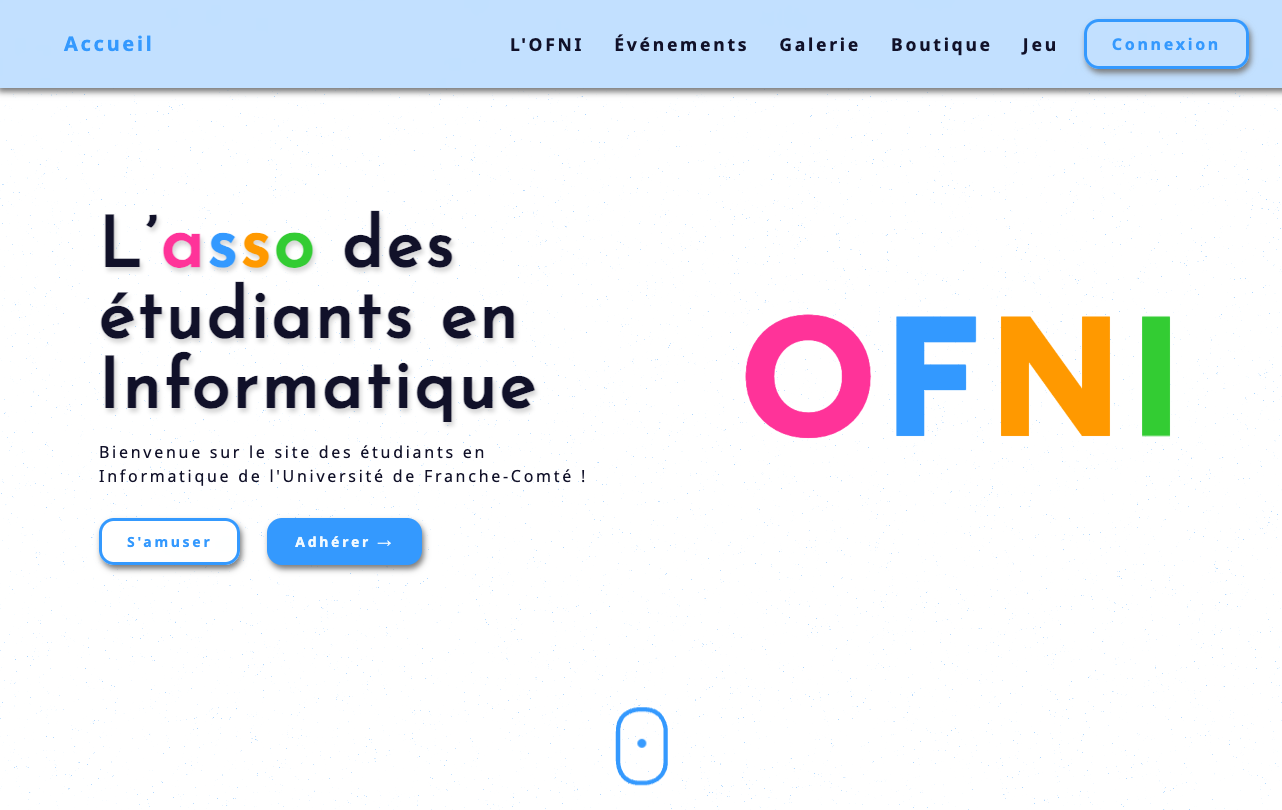
\includegraphics[width=\textwidth]{assets/pictures/home-page.png}
    \caption{Page d'accueil du site de l'\ofni}
    \label{fig:home-page}
\end{figure}

Le site contient un certain nombre de pages de formalités, qui sont des pages statiques pour la plupart. On y trouve notamment l'accueil du site, que l'on peut voir \figureref{fig:home-page}, la page de présentation de l'association, celle d'adhésion ainsi que celle des mentions légales. Certaines de ces pages sont présentent des informations qu'il est, juridiquement, obligatoire de faire apparaître sur un site web. C'est le cas des mentions légales, qui sont des informations sur l'association, son siège social, son numéro de téléphone, son adresse \langue{e-mail}, son numéro de \logo{SIRET}, etc.

Il est tout de même possible de trouver un petit peu de dynamisme sur certaines pages, notamment la page d'accueil qui contient des petits \langue{teasers} sur les activités à venir de l'association, ou encore des actualités.

\subsection{Le jeu \game}
\label{subsec:jeu}

% game screenshot
\begin{figure}[h]
    \centering
    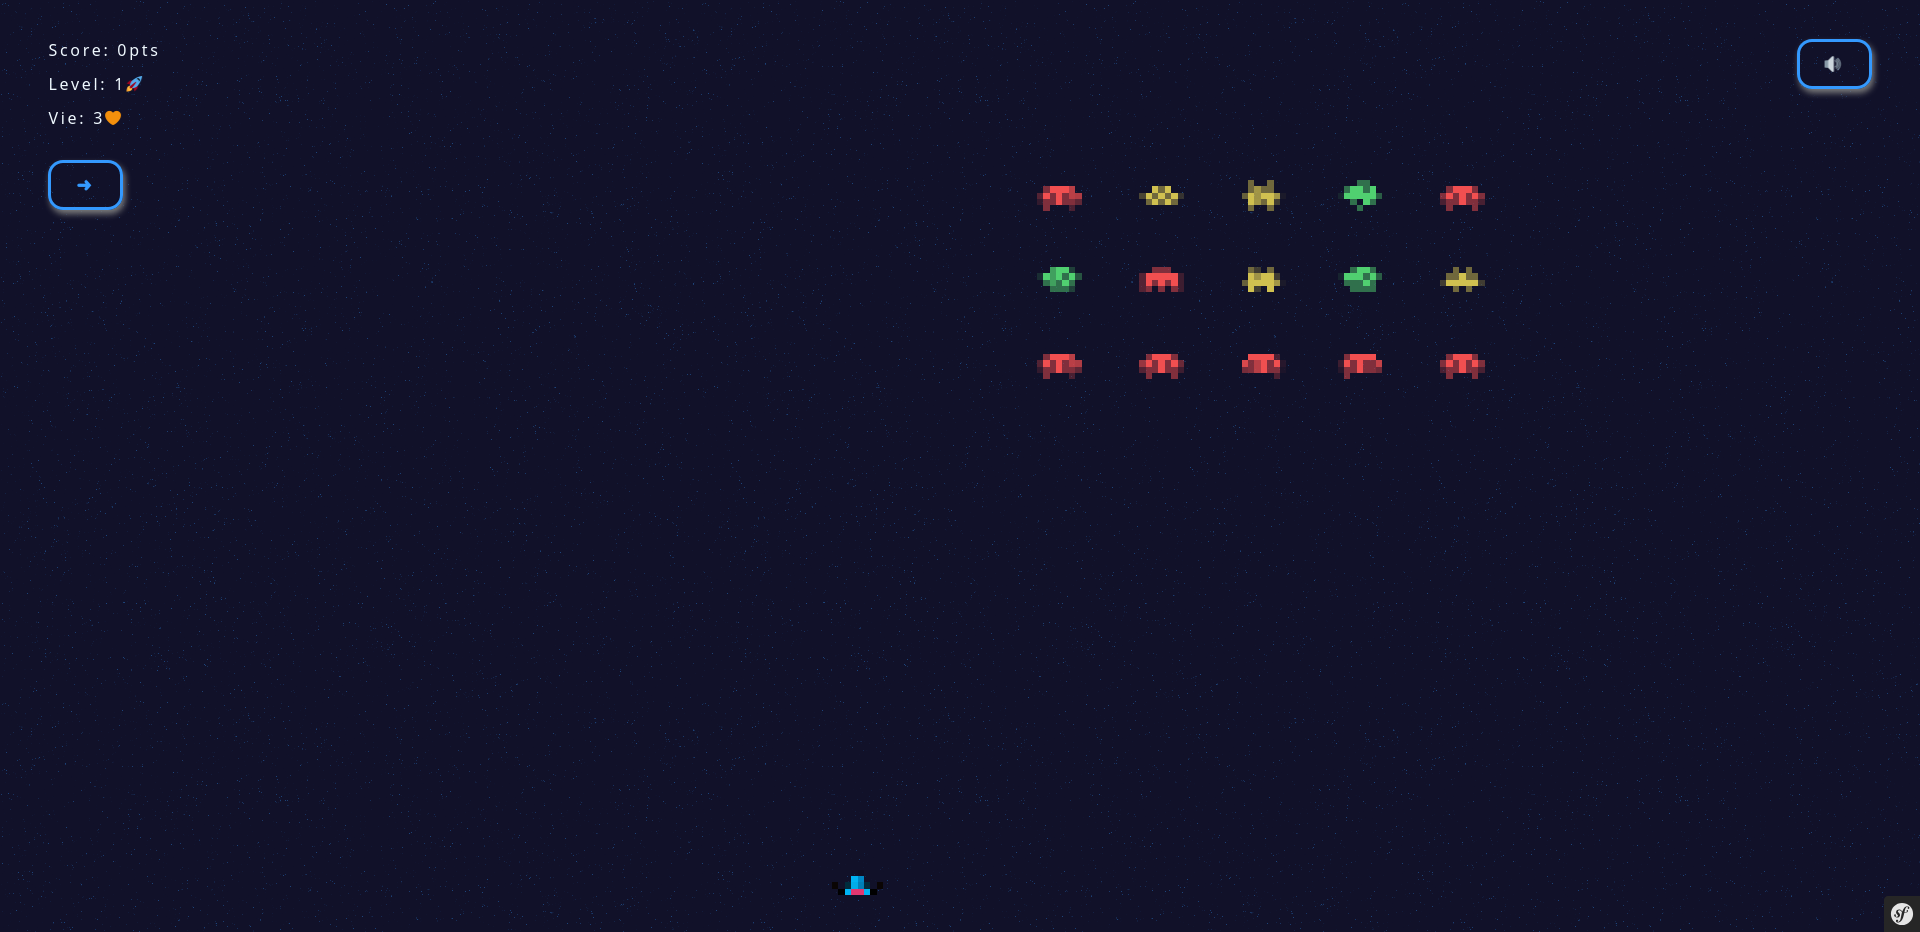
\includegraphics[width=\textwidth]{assets/pictures/game.png}
    \caption{Vue du jeu \game}
    \label{fig:game}
\end{figure}

Peu avant le début de la phase de développement, il fut décider d'ajouter un petit jeu vidéo au site avec un afficage du meilleur joueur pour rendre la visite du site plus attractive. Le jeu \game\ est un jeu de type \citer{Space Invaders} où le joueur doit tirer sur des vaisseaux ennemis pour marquer des points. Le jeu est jouable directement depuis le site, sans avoir besoin de télécharger quoi que ce soit. On peut voir une capture d'écran du jeu \game\ en \figureref{fig:game}.

\subsection{La connexion et l'inscription aux événements}
\label{subsec:connexion-inscription}

Ces actualités et événements de l'\ofni\ constitue la partie centrale du site. Tout cela commence évidemment par un page de connexion, ou de création de compte si l'utilisateur n'en a pas encore. Une fois connecté, l'utilisateur peut alors s'inscrire à des événements.

Comme vu dans la section \ref{subsec:generation-formulaire}, les formulaires d'inscription aux événements sont générés automatiquement à partir des informations de la base de données. Cela permet de ne pas avoir à modifier le code du site à chaque nouvel événement ou bien de réutiliser un même formulaire pour plusieurs éditions.
\bigskip

Lorsque l'administrateur décide de créer un nouveau formulaire, il va en réalité définir ce qui, dans la terminologie du présent site, s'appelle un \formwidget. Il existe trois types de \formwidget\ différents~:
\begin{description}
    \item[Natif] Qui correspond à un champ simple, comme par exemple un texte, une date, ou encore une case à cocher. Ils sont définis par défaut dans le site et ne peuvent pas être modifiés ou ajoutés par l'administrateur. Ils sont les briques fondamentales pour la construction d'autres \formwidget\ plus avancés.
    \item[Composite] Un ensemble de \formwidget\ les uns à la suite des autres. Par exemple, un \formwidget\ composite pourrait être un \formwidget\ natif de type text, suivi d'un \formwidget\ natif de type date, puis d'un autre \formwidget\ composite défini en amont. Ils sont définis par l'administrateur et peuvent être réutilisés dans d'autres \formwidget.
    \item[Liste] Un ensemble de taille indéfinie de \formwidget\ de même type, mais qui peuvent être répétés autant de fois que nécessaire. Par exemple, un \formwidget\ liste pourrait être un \formwidget\ composite décrivant un membre d'une équipe ; l'utilisateur peut alors, lors de son inscription, en remplir autant de fois qu'il ne le faut pour que tous les membres du groupe soient enregistrés. Ils sont définis par l'administrateur et peuvent être réutilisés dans d'autres \formwidget.
\end{description}

Lorsque l'utilisateur s'inscrit à un événement, le formulaire, correspondant à un \formwidget, est alors généré dynamiquement. Il est alors possible de définir des formulaires très complexes, avec des champs de différents types, des champs répétables, etc.

\section{Les fonctionnalités non implémentées}
\label{sec:non-implem}

Il est important de noter que tout n'a pas été implémenté. Les différentes réunions de travail ont permis de définir les priorités et de déterminer ce qui était le plus important pour le site. Certaines fonctionnalités ont alors été retirées pour cause d'une utilité moindre ou d'une impossibilité à les commencer, tandis que d'autres ont été ajoutées en cours de développement.
\bigskip

On peut par exemple noter qu'au départ, il fut prévu que le système de connexion passe par le \logo{CAS} officiel de l'\univ. Cependant, les demandes d'autorisation pour utiliser ces systèmes n'ayant pas abouti, l'idée a dû finalement être abandonnée. Il en est de même pour la gestion des utilisateurs, qui devait être faite par le \logo{CAS}.

Mais au-delà des restrictions administratives, d'autres fonctionnalités n'ont pas vu le jour par pure manque de temps. C'est par exemple le cas du \citer{Crochet \logo{Discord}}, qui devait permettre de diffuser automatiquement les événements de l'\ofni\ sur le serveur \logo{Discord} de l'association dès la création de l'événement sur le site.

\section{Ambitions pour l'avenir du site}
\label{sec:avenir}

Certes, tout n'est pas implémenté. À ce jour, le site est fonctionnel et permet de remplir les objectifs principaux qui lui ont été fixés. Ajoutant en plus certaines fonctionnalités comme \game. Il est alors naturel de se demander quelles sont les prochaines pistes d'amélioration pour le site.
\bigskip

On pense en tout premier lieu aux \langue{features} qui ne sont pas contraintes administrativement, comme le \citer{Crochet \logo{Discord}} vu précédemment dans la section \ref{sec:non-implem}.

Mais même du côté de ce qui fonctionne, on peut aussi y voir des pistes d'amélioration majeures, en particulier concernant la partie \logo{CMS}. En effet, pour la génération de formulaires, nous avons vu section \ref{subsec:connexion-inscription} que les \formwidget\ natifs étaient là par défaut et ne pouvaient, ni être modifiés, ni être ajoutés. Il serait alors intéressant de permettre à l'administrateur de créer ses propres \formwidget\ natifs, pour pouvoir les réutiliser dans d'autres \formwidget\ plus complexes. Cela peut par exemple passer par la définition d'une \logo{Regex} par l'administrateur. Cette \logo{Regex} permettrait alors de valider ou non le champ de texte lors de la soumission du formulaire par l'utilisateur.
\bigskip

D'un point de vue du développement, il peut également être judicieux de rédiger une documentation encore plus complète pour les futurs bureaux qui souhaiteraient reprendre le projet. Cela permettrait de faciliter la prise en main du site et de garantir une continuité dans son développement.
